\documentclass{article}
\usepackage[utf8]{inputenc}
\usepackage{listings}
\usepackage{graphicx}
\usepackage{float}
\usepackage{xcolor}
\usepackage{geometry}
\usepackage{CJKutf8}
\usepackage{amsmath}
\usepackage{amssymb}

\geometry{a4paper,scale=0.8}
\lstset{
    basicstyle          =   \sffamily,        
    keywordstyle        =   \bfseries,         
    commentstyle        =   \rmfamily\itshape, 
    stringstyle         =   \ttfamily, 
    flexiblecolumns,               
    numbers             =   left,  
    showspaces          =   false, 
    showstringspaces    =   false,
    captionpos          =   t,     
    frame               =   lrtb, 
}

\lstdefinestyle{Python}{
    language        =   Python, % 语言选Python
    basicstyle      =   \zihao{-5}\ttfamily,
    numberstyle     =   \zihao{-5}\ttfamily,
    keywordstyle    =   \color{blue},
    keywordstyle    =   [2] \color{teal},
    stringstyle     =   \color{magenta},
    commentstyle    =   \color{red}\ttfamily,
    breaklines      =   true,  
    columns         =   fixed,  
    basewidth       =   0.5em,
}

\title{\bf\Large  概率论与数理统计 第4次作业}
%%%%%%%%%%%%%%%%%%%%%%%%%%%%%%%%%%%%%%
%% DON'T forget to change this part %%
\author{\bf Name: 宋昊原 \qquad Student ID: 2022010755}
%%%%%%%%%%%%%%%%%%%%%%%%%%%%%%%%%%%%%%

\begin{document}
\begin{CJK}{UTF8}{gbsn}
\maketitle
\section{掷6颗骰子}
设$X$为出现的1点的数量,则$X\sim B(6,\frac{1}{6})$,概率精确值为
$$ P(X=2)=\tbinom{6}{2}(\frac{1}{6})^{2}(\frac{5}{6})^{4}=0.2009 $$
利用Poisson分布$P(1)$近似,则
$$ P(X=2)=\frac{1^{2}}{2!}e^{-1}=0.1839 $$
\section{访问网站}
设$X$为访问该网站的人数,则$X\sim B(10^{6},2\times 10^{-6})$,概率精确值为
$$ P(X=2)=\tbinom{10^{6}}{2}(2\times 10^{-6})^{2}(1-2\times 10^{-6})^{10^{6}-2}=0.2707$$
利用$P(2)$近似,则
$$ P(X=2)=\frac{2^{2}}{2!}e^{-2}=0.2707 $$
二者非常接近
\section{昆虫后代}
设产卵数为$X$,后代数为$Y$,$n$个卵产生$m$个后代的概率为$f(n,m)$,由题意,$X\sim P(\lambda)$,
$$ P(X=n)=\frac{\lambda^{n}}{n!}e^{-\lambda}$$
$$ f(n,m)=P(Y=m|X=n)=\tbinom{n}{m}p^{m}(1-p)^{m} $$
则根据全概率公式,
$$ P(Y=k)=\sum\limits_{i=k}^{\infty}P(X=i)f(i,k)$$
$$ =\sum\limits_{i=k}^{\infty}\frac{\lambda^{i}e^{-\lambda}i!p^{k}(1-p)^{i-k}}{i!k!(i-k)!}$$
$$ =\frac{(\lambda p)^{k}e^{-\lambda}}{k!}\sum\limits_{i=k}^{\infty}\frac{(\lambda(1-p))^{i-k}}{(i-k)!}$$
$$ =\frac{(\lambda p)^{k}e^{-\lambda}}{k!}\sum\limits_{i=0}^{\infty}\frac{(\lambda(1-p))^{i}}{(i)!}$$
$$ =\frac{(\lambda p)^{k}e^{-\lambda}}{k!}\times e^{\lambda(1-p)}$$
$$ =\frac{(\lambda p)^{k}e^{-\lambda p}}{k!} $$
故$Y\sim P(\lambda p)$.
\section{已知期望求参数}
先考虑归一化条件.
$$ \int_{0}^{1}f(x)dx=\int_{0}^{1}(a+bx^{2})dx $$
$$ =(ax+\frac{1}{3}bx^{3})|_{0}^{1}$$
$$ =a+\frac{b}{3}=1$$
再考虑期望
$$ E(X)=\int_{0}^{1}xf(x)dx$$
$$ =\int_{0}^{1}(ax+bx^{3})dx$$
$$ =(\frac{1}{2}ax^{2}+\frac{1}{4}bx^{4})|_{0}^{1}$$
$$ =\frac{a}{2}+\frac{b}{4}=\frac{2}{3} $$
解此方程组,得
$$ a=\frac{1}{3}$$
$$ b=2$$
\section{等待时间}
以10点为0时刻,1分钟为单位时间,定义该参观者到馆时间为$X$,则其PDF为
\begin{equation}
    f(x)=\left\{
    \begin{array}{cl}
    \frac{1}{60} & 0<x<60\\
    0 & else\\
    \end{array}\right.
\end{equation}
\subsection{}
$$ P(20\leq x\leq 30 \lor 50\leq x<60)=\frac{20}{60}=\frac{1}{3} $$
\subsection{}
$$ P(0<x<10 \lor 30<x<40)=\frac{20}{60}=\frac{1}{3}$$
\section{怀孕天数}
怀孕天数$X\sim N(270,100)$,其PDF为
$$ f(x)=\frac{1}{\sqrt{200\pi}}e^{-\frac{(x-270)^{2}}{200}}$$
故
$$ P(240<X<290)=\int_{240}^{290}f(x)dx=0.9759$$
则
$$ P(X\leq 240 \lor X\geq 290)=1-P(240<X<290)=0.0241$$
\section{电池续航}
\subsection{指数分布}
服从指数分布时,从任意时刻开始计时得到的分布是一样的,因此可以直接从当前时刻考虑还能继续跑的万公里数$X$,则
$$ X\sim Exp(\frac{1}{3})$$
于是
$$ P(X\geq 1)=1-F(1)=e^{-\frac{1}{3}\times 1}=0.7165$$
\subsection{非指数分布}
如果不服从指数分布,那么从任意时刻开始计时得到的分布不一定一样,必须从电池无损耗的时刻开始计时,考虑此时还能继续跑的万公里数$Y$,则所求概率为
$$ P(Y\geq 2.5|Y\geq 1.5)=\frac{P(Y\geq 2.5)}{Y\geq 1.5}=\frac{1-F(2.5)}{1-F(1.5)}$$
\section{法官决策}
\subsection{}
以95\%的把握不冤枉无罪的人意味着无罪的人被判有罪的概率为5\%.
设无罪的人的该证据为$X$,则$X\sim Exp(1)$,则原条件为
$$ P(X>c)=e^{-c}=0.05 $$
即
$$ c=-\ln 0.05=2.996 $$
\subsection{}
设有罪的人该证据为$Y$,则$Y\sim Exp(\frac{1}{2})$,则
$$ P(Y>c)=e^{-\frac{c}{2}}=0.2236 $$
即有罪的人被判为有罪的概率也只有22.36\%.
\section{对数正态分布}
这里对数按自然对数$\ln$处理. 设$X=\ln Y$,则$X\sim N(\mu,\sigma^{2})$. 设$X$的CDF和PDF分别为$F$和$f$,$Y$的CDF和PDF分别为$G$和$g$,则
$$ f(x)=\frac{1}{\sqrt{2\pi}\sigma}e^{-\frac{(x-\mu)^{2}}{2\sigma^2}}$$
于是
$$ F(x)=\int_{-\infty}{x}f(t)dt $$
由于
$$ P(Y\leq y)=P(X\leq \ln y)$$
故
$$ G(y)=F(\ln y)=\int_{-\infty}{\ln y}f(t)dt $$
对$y$求导,有
$$ g(y)=\frac{1}{y}f(\ln y)=\frac{1}{\sqrt{2\pi}\sigma y}e^{-\frac{(\ln y-\mu)^{2}}{2\sigma^{2}}}$$
此即$Y$的概率密度函数.
\section{随机变量的函数}
\subsection{}
先考虑$g(X)$的累积分布函数,设为$G(y)$,设$g(x)$严格单调递增且可微,则
$$ G(y)=P(Y\leq y)=P(g(X)\leq y)=P(X\leq g^{-1}(y))=F(g^{-1}(y))$$
由于$F$连续且$X$有PDF,$F$可微,同时$g^{-1}$可微,于是$G$可微,进而$g(X)$有PDF:
$$h(y)=\frac{d}{dy}G(y)=\frac{F'(g^{-1}(y))}{g'(g^{-1}(y))}$$
此时对于任何使$f(x)=f(g^{-1}(y))$连续的点,都有$F'(g^{-1}(y))=f(g^{-1}(y))$,故在这些点(几乎全部的点)有
$$h(y)=\frac{f(g^{-1}(y))}{g'(g^{-1}(y))}$$
若$g(x)$单调递减,则类似地,有
$$ G(y)=P(Y\leq y)=P(g(X)\leq y)=P(X\geq g^{-1}(y))=1-F(g^{-1}(y))$$
$$h(y)=-\frac{f(g^{-1}(y))}{g'(g^{-1}(y))}$$
注意:上述讨论仅限$g(x)$值域内的范围,对于其他可能的取值,$g(X)$的PDF显然应取0.
\subsection{}
$F(x)$连续且严格单调,故存在反函数. 设$Y=F(x)$的CDF为$G(y)$,则
$$ G(y)=P(Y\leq y)=P(F(X)\leq y)=P(X\leq F^{-1}(y))=F(F^{-1}(y))=y$$
考虑到上述讨论中$Y=F(X)$的范围是$[0,1]$,于是
\begin{equation}
    G(y)=\left\{
    \begin{array}{cl}
    0 & y<0\\
    y & 0\leq y\leq 1\\
    1 & y>1\\
    \end{array}\right.
\end{equation}
这是$[0,1]$上的均匀分布.
\subsection{}
先证明结论.
$F^{-1}(Y)$的累积分布函数$F_{1}(x)$满足
$$ F_{1}(x)=P(F^{-1}(Y)\leq x)=P(Y\leq F(x)) $$
由于$Y\sim U(0,1)$且$F(x)\in [0,1]$,于是
$$P(Y\leq F(x))=F(x)$$
于是
$$ F_{1}(x)=F(x)$$
证毕.
\\\\下面给出说明
\\设$F(x)=1-e^{-\lambda x}(x\geq 0)$,则$F^{-1}(y)=-\frac{\ln(1-y)}{\lambda}$.
\\这说明,若$Y\sim U(0,1)$,则$F^{-1}(Y)=-\frac{\ln(1-Y)}{\lambda}\sim Exp(\lambda)$.
\subsection{}
此结论给出了一种把均匀分布通过随机变量的函数变换为其他分布的方式.
\subsection{}
去除此假设后(2)的结论不再正确. 反例如下:
\begin{equation}
    F(x)=\left\{
    \begin{array}{cl}
    0 & x<0\\
    1 & x\geq 1\\
    \end{array}\right.
\end{equation}
即,$X$总是取1,那么相应地,$Y=F(X)$也只能取$F(1)=1$.
\\进一步地讲,$X$是离散随机变量时,$Y=F(X)$不可能是连续的均匀分布.
\section{从连续到离散}
\subsection{}
$Y$是离散的,求其PMF.
\\设$I_{i}$的左端点为$t_{i-1}$,右端点为$t_{i}$,则$p_{i}=t_{i}-t_{i-1}$.
$$ f(i)=P(Y=i)=P(t_{i-1}<X<t_{i})=t_{i}-t_{i-1}=p_{i}$$
\subsection{}
可以.
\\对于任何一离散型随机变量$Y$,设其可能取值$y_{1},y_{2},...$的概率分别为$p_{1},p_{2},...$,则有
$$\sum\limits_{i=1}^{\infty}p_{i}=1$$
此时令$X\sim U(0,1)$,$Y'$与$X$有如下函数关系:
$$ Y'=y_{i}\iff \sum\limits_{j=1}^{i-1}p_{j}\leq X<\sum\limits_{j=1}^{i}p_{j}$$
这样构造的$Y'$与前面的$Y$同分布.
\section{随机分线段}
令$X$为断点的位置,$Y$为含$p_{0}$的那一段的长度,则
$$ X\sim U(0,1)$$
\begin{equation}
    Y=\left\{
    \begin{array}{cl}
    1-X & 0\leq X\leq p_{0}\\
    X & X>p_{0}\\
    \end{array}\right.
\end{equation}
于是期望
$$ E(Y)=\int_{0}^{p_{0}}(1-x)dx+\int_{p_{0}}^{1}xdx$$
$$ =(x-\frac{x^{2}}{2})|_{0}^{p_{0}}+\frac{x^{2}}{2}|_{p_{0}}^{1}$$
$$ =p_{0}-\frac{p_{0}^{2}}{2}+\frac{1}{2}-\frac{p_{0}^{2}}{2}$$
$$ =-p_{0}^{2}+p_{0}+\frac{1}{2}$$
\section{条件概率分布}
\textbf{引理}
\\若$A_{1},A_{2},...,A_{n}$是样本空间的一个划分,且在$A_{i}$发生的条件下$X$的PDF为$f_{i}(x)$,则$X$的PDF为
$$ f(x)=\sum\limits_{i=1}^{n}P(A_{i})f_{i}(x)$$
\\\\
\textbf{引理证明}\\
$\forall I\subset\mathbb{R}\land I$可测,根据全概率公式有
$$ P(X\in I)=\sum\limits_{i=1}^{n}P(A_{i})P(X\in I|A_{i})=\sum\limits_{i=1}^{n}P(A_{i})\int_{I}f_{i}(x)dx=\int_{I}(\sum\limits_{i=1}^{n}P(A_{i})f_{i}(x))dx=\int_{I}f(x)dx$$
由PDF的定义,引理得证.
\\\\
于是,很容易得出此题中$X$的PDF:
\begin{equation}
    f(x)=\left\{
    \begin{array}{cl}
    \frac{1}{2} & 0\leq X<1\lor 3\leq X<4\\
    0 & else\\
    \end{array}\right.
\end{equation}
故
$$E(X)=\int_{0}^{1}\frac{1}{2}xdx+\int_{3}^{4}\frac{1}{2}xdx=2$$
$$Var(X)=\int_{0}^{1}\frac{1}{2}(x-2)^{2}dx+\int_{3}^{4}\frac{1}{2}(x-2)^{2}dx=\frac{7}{3}$$
\section{$\beta$分布}
$\beta$分布是二项分布的共轭先验分布,即它给出了在已知二项分布测试结果但不知参数$p$时对其的一种预测. \\其PDF为:
$$ f(x)=\frac{x^{\alpha-1}(1-x)^{\beta-1}}{\int_{0}^{1}u^{\alpha-1}(1-u)^{\beta-1}du}=\frac{x^{\alpha-1}(1-x)^{\beta-1}}{B(\alpha,\beta)},x\in(0,1)$$
其期望
$$ E(X)=\int_{0}^{1}xf(x)dx=\frac{1}{B(\alpha,\beta)}\int_{0}^{1}x^{\alpha}(1-x)^{\beta-1}dx=\frac{B(\alpha+1,\beta)}{B(\alpha,\beta)}=\frac{\alpha}{\alpha+\beta} $$
考虑平方的期望
$$ E(X^{2})=\int_{0}^{1}x^{2}f(x)dx=\frac{1}{B(\alpha,\beta)}\int_{0}^{1}x^{\alpha+1}(1-x)^{\beta-1}dx=\frac{B(\alpha+2,\beta)}{B(\alpha,\beta)}=\frac{\alpha(\alpha+1)}{(\alpha+\beta)(\alpha+\beta+1)}$$
故方差
$$ Var(X)=E(X^{2})-E^{2}(X)=\frac{\alpha(\alpha+1)}{(\alpha+\beta)(\alpha+\beta+1)}-\frac{\alpha^{2}}{(\alpha+\beta)^{2}}$$
$$ =\frac{\alpha(\alpha+1)(\alpha+\beta)-\alpha^{2}(\alpha+\beta+1)}{(\alpha+\beta)^{2}(\alpha+\beta+1)}$$
$$ =\frac{\alpha^{3}+\alpha^{2}+\alpha^{2}\beta+\alpha\beta-\alpha^{3}-\alpha^{2}\beta-\alpha^{2}}{(\alpha+\beta)^{2}(\alpha+\beta+1)}$$
$$ =\frac{\alpha\beta}{(\alpha+\beta)^{2}(\alpha+\beta+1)}$$
\section{计算机实验:正态分布}
\subsection{}
1000个正态随机数的直方图如下:
\\
\begin{minipage}{0.5\textwidth}
    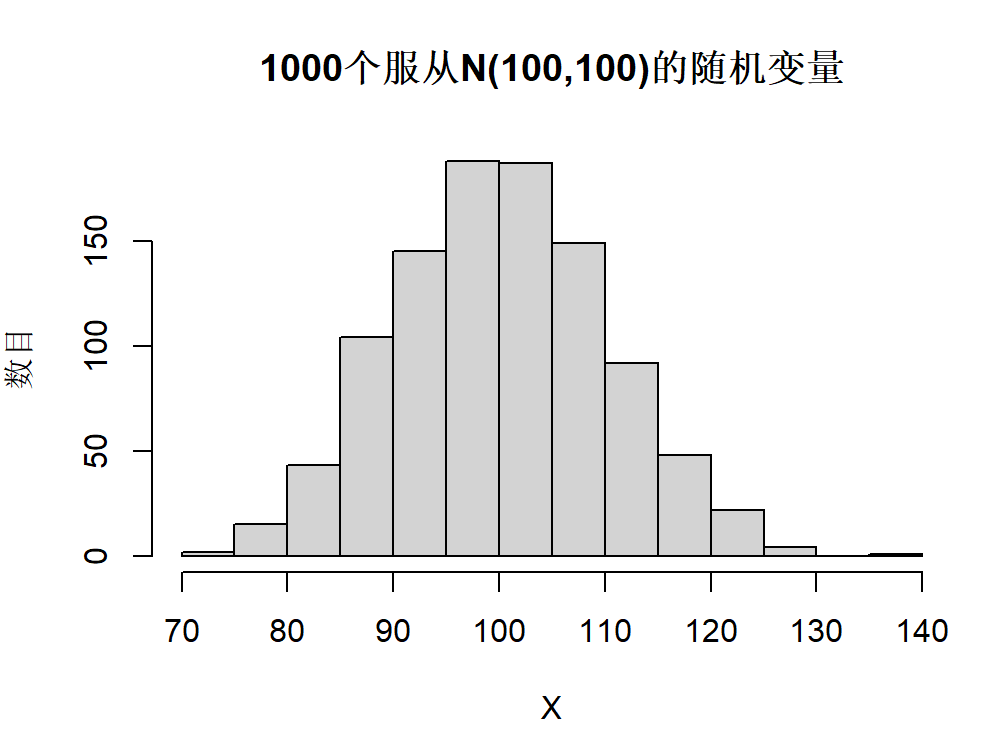
\includegraphics[scale=0.6]{hist1.png}
\end{minipage}
\subsection{}
从上述1000个随机数中抽取1000个样本的直方图如下:
\\
\begin{minipage}{0.5\textwidth}
    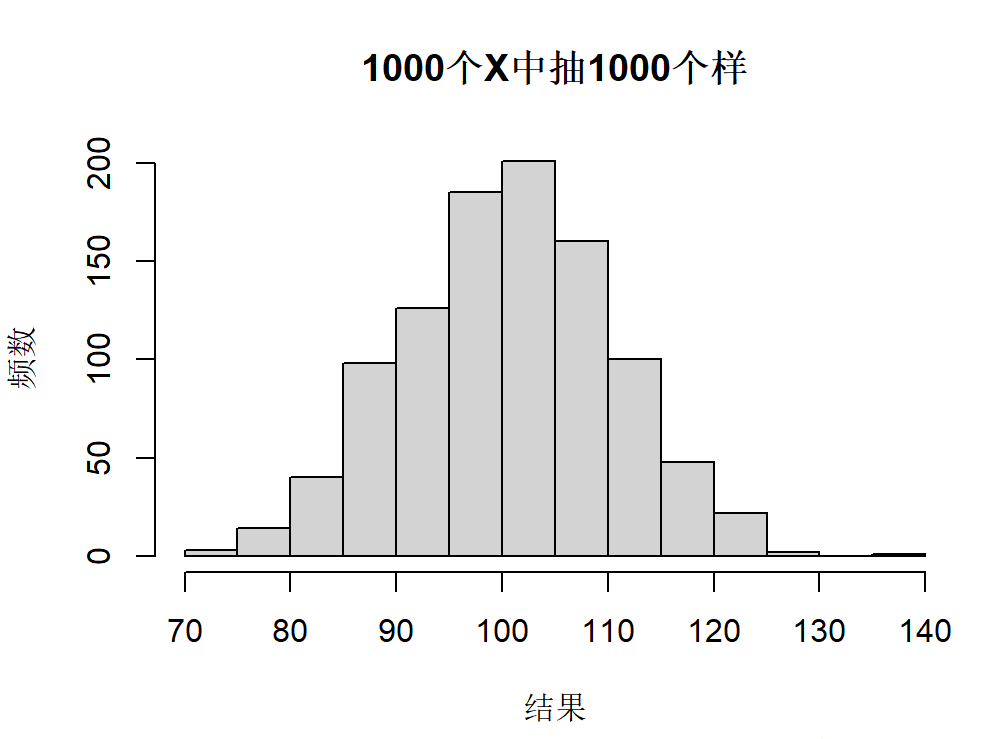
\includegraphics[scale=0.6]{hist2.png}
\end{minipage}
\subsection{}
第一个样本均值为100.2348,方差为99.41973.
\\第二个样本均值为100.6543,方差为95.92514.
\\二者的均值和方差比较接近
\subsection{}
本题使用代码如下:
\\
\begin{minipage}{0.5\textwidth}
    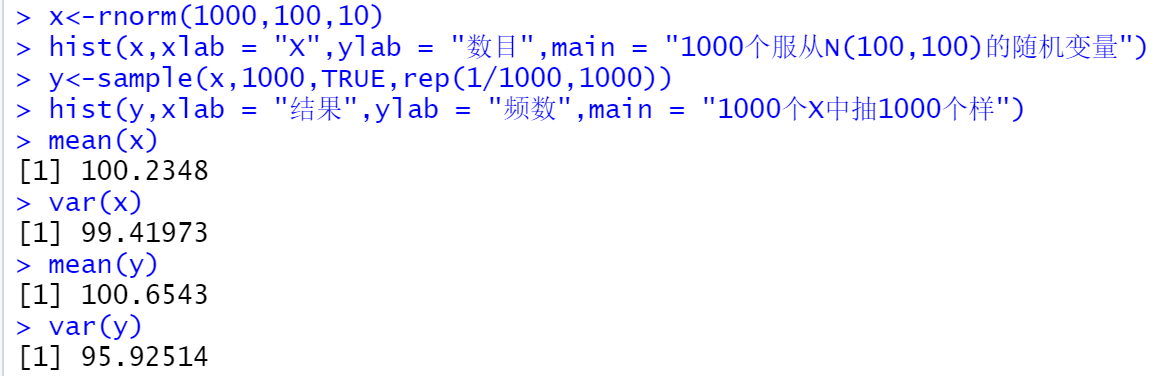
\includegraphics[scale=0.6]{code.png}
\end{minipage}
\end{CJK}
\end{document}